\documentclass{beamer}
\usepackage{tikz}
\usepackage{fancyvrb}
\title{Attacks on Block Cipher Modes of Operation\\RPISEC}
\date{November 11, 2016}
\author{Avi Weinstock (\Verb|aweinstock|), Adam Freeman (\Verb|triazo|)}
\begin{document}
\maketitle

\begin{frame}[fragile]
\frametitle{Setup}
\begin{itemize}
\item Python libraries: \verb|sudo pip install pycrypto pwntools|
\item
\verb|pycrypto| is practically required, \verb|pwntools| is merely recommended.
\item \verb|triazo| is currently hosting the challenges at \verb|http://blackbox.rpi.rip/|
\item You can get an offline copy of the challenges from \verb|https://github.com/pbiernat/BlackBox|
\end{itemize}
\end{frame}

\begin{frame}[fragile]
\frametitle{What is a Block Cipher?}
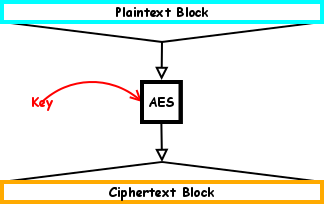
\includegraphics[width=0.9\textwidth]{diagram_images/SingleBlock.png}\\
\end{frame}

\begin{frame}[fragile]
\frametitle{Electronic Code Book (ECB)}
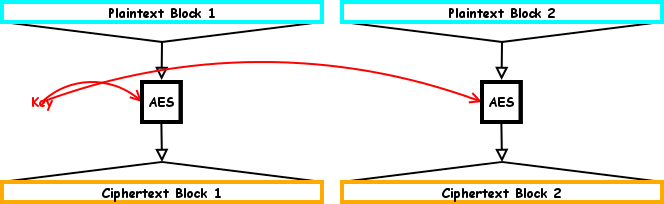
\includegraphics[width=0.9\textwidth]{diagram_images/ECB.png}\\
\end{frame}

\begin{frame}[fragile]
\frametitle{Counter (CTR)}
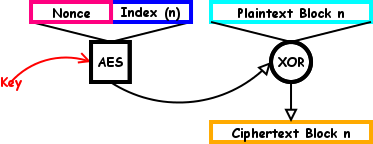
\includegraphics[width=0.9\textwidth]{diagram_images/CTR.png}\\
\end{frame}

\begin{frame}[fragile]
\frametitle{Cipher Block Chaining (CBC)}
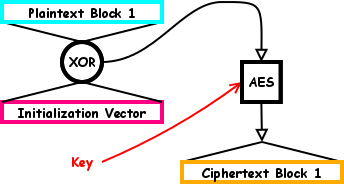
\includegraphics[width=0.9\textwidth]{diagram_images/CBC.png}\\
\end{frame}

\begin{frame}[fragile]
\frametitle{Cipher Block Chaining (CBC)}
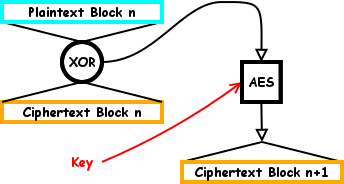
\includegraphics[width=0.9\textwidth]{diagram_images/CBC_Induction.png}\\
\end{frame}

\begin{frame}[fragile]
\frametitle{Resources}
\begin{itemize}
\item \verb|https://en.wikipedia.org/wiki/Block_cipher|
\item \verb|https://en.wikipedia.org/wiki/|\\\verb|Block_cipher_modes_of_operation|
\item \verb|https://cryptopals.com/|
\end{itemize}
\end{frame}
\end{document}
